\documentclass{article}
\usepackage{graphicx} % Required for inserting images
\usepackage{amsmath,amssymb}
\usepackage{url}
\usepackage{xcolor}


\title{The (analytic) halo model vs.\ PT/EFT}
\author{Martin White}
\date{Notes}

\begin{document}

\maketitle

\section{Introduction}

The halo model is a useful tool for understanding the clustering of objects in the Universe, and has been used to try to understand the non-linear regime of clustering.  The halo model exists in `weak' and `strong' forms, and as a recipe for placing objects in N-body simulations or an analytic theory.  The analytic version of the model provides a useful structure for thinking about
gravitational clustering and gives multiple insights, but it also has numerous well-documented problems both conceptually and phenomenologically.
The purpose of this note is to look at the ``analytic'' halo model vs.\ perturbation theory (a.k.a.\ effective field theory) for Einstein-de Sitter cosmologies with power-law initial power spectra.  Our focus will be on very ``red'' spectra where the approach to non-linearity behaves very differently in perturbation theory and the halo model.

\section{Scale free cosmologies}

Since classical gravity has no explicit scale, the evolution of clustering in an Einstein-de Sitter ($\Omega_m=1$) cosmology with an initially power-law power spectrum would be expected to be self-similar or scale-free.  Henceforth we shall assume $\Omega_m=1$ and take the initial power spectrum to be a power law with index $n$, $P\propto k^n$.  Specifically, in terms of the dimensionless power, we choose
\begin{equation}
    \Delta_{\rm lin}^2(k) \equiv \frac{k^3\,P(k)}{2\pi^2}
    = \left(\frac{k}{k_\star}\right)^{3+n} = \kappa^{3+n}
    \qquad (-3<n<-1)
\end{equation}
where we have defined a dimensionless wavenumber, $\kappa=k/k_\star$.
The time evolution of the power spectrum can be traded for scale dependence such that the evolved power spectrum is a fixed function of $k\,a^{2/(3+n)}$:
\begin{equation}
    \Delta^2(k,a) = F\left( k\, a^{2/(3+n)} \right) 
\end{equation}
For the rest of this paper we shall take $a=1$ and we shall primarily be interested in $\kappa<1$.

\section{N-body}

We have measured the dimensionless power spectra from Fig.~1 of \url{https://arxiv.org/pdf/2109.04397}.  These data have been read from the figures and are notably noisy at low $k$, but in that regime we know the theory is very accurate.

\section{Perturbation theory}

The 1-loop power spectrum for power-law cosmologies has been known for many years (\url{https://arxiv.org/pdf/astro-ph/9602070}; Appendix B\footnote{This reference uses a $2\pi$ convention where $\Delta^2=4\pi\,k^3\,P(k)$.  We have converted where necessary.}).  It has
\begin{equation}
    \Delta^2(k) = \kappa^{3+n} + a_n^\mathrm{PT} \kappa^{2(3+n)} + \alpha\, \kappa^{5+n}
\end{equation}
where we have added the lowest-order counterterm from integrating out small-scale physics.  The coefficient, $\alpha$, of this counterterm needs to be fit to data or simulations and is expected to be $\mathcal{O}(1)$.  Note that since $n<-1$ the counterterm is more suppressed than the 1-loop term when $\kappa\ll 1$.

The value of $a_n^{\rm PT}$ can be expressed as a sum of ratios of $\Gamma$ functions depending only upon $n$.  Numerical values are given in Table \ref{tab:numbers} for several values of $n$.

\begin{table}
    \centering
    \begin{tabular}{cccccc}
    $n$ & $3+n$ & $a_n^\mathrm{PT}$ & $a_n^\mathrm{HM}$ & $\kappa_{10}^\mathrm{PT}$ & $\kappa_{10}^\mathrm{HM}$ \\ \hline
    $-5/4$ & $7/4$ &$-0.4005$ & $0.2444$ & $0.450$ & $0.489$ \\
    $-3/2$ & $3/2$ & $0.2052$ & $0.2816$ & $0.617$ & $0.502$ \\
    $-7/4$ & $5/4$ & $0.6963$ & $0.4052$ & $0.211$ & $0.450$ \\
    $-2$   & $1$   &  $1.385$ & $0.9282$ & $0.072$ & $0.328$ \\
    $-17/8$& $7/8$ &  $1.890$ & $1.984$  & $0.035$ & $0.245$ \\
    $-9/4$ & $3/4$ &  $2.582$ & $6.534$  & $0.013$ & $0.156$ \\
    $-19/8$& $5/8$ &  $3.577$ & $46.23$  & $0.003$ & $0.076$ \\
    $-5/2$ & $1/2$ &  $5.104$ & $1454$   & --      & $0.022$ \\ \hline
    \end{tabular}
    \caption{Key quantities as a function of the power-law index, $n$.  $a_n^\mathrm{PT}$ is the coefficient of the 1-loop power spectrum ($\kappa^{2(3+n)}$), $a_n^\mathrm{HM}$ is the amplitude of the 1-halo term ($\kappa^3$), and $\kappa_{10}^\mathrm{PT}$ is where $|P_{\rm 1-loop}|/P_{\rm tree}=10\%$ while $\kappa_{10}^\mathrm{HM}$ is where $P_{\rm 1-halo}/P_{\rm 2-halo}=10\%$.}
    \label{tab:numbers}
\end{table}

\section{Halo model}

The halo model postulates that on large scales dark matter halos cluster according to linear theory while on small scales the power is dominated by the halo profiles. Specifically most pairs of dark matter particles with small interparticle separations lie within the same halo, and thus their correlations can be predicted by the halo profile.

The halo model, in this simplest, analytic form, for scale-free cosmologies has been worked out in \url{https://arxiv.org/pdf/astro-ph/0510100} .  In the limit where we can neglect the halo profiles ($y\approx 1$; valid for $\kappa\ll 1$ or $k\,r_{\rm vir}\ll 1$ for $M_\star$ halos),
\begin{equation}
  \Delta^2 = \kappa^{3+n} +  a_n^\mathrm{HM} \kappa^3
  \qquad (y \approx 1)
\end{equation}
where $a_n^\mathrm{HM}$ is known analytically in terms of $\Gamma$ functions (\url{https://arxiv.org/pdf/astro-ph/0510100}) and depends only upon $n$.  Some numerical values are tabulated in Table \ref{tab:numbers} for specific values of $n$.
Note that the 1-halo term has the same slope as the 1-loop power spectrum for $n=-3/2$ and as the counterterm for $n=-2$.

\section{Comparison}

\begin{figure}
    \centering
    \resizebox{\columnwidth}{!}{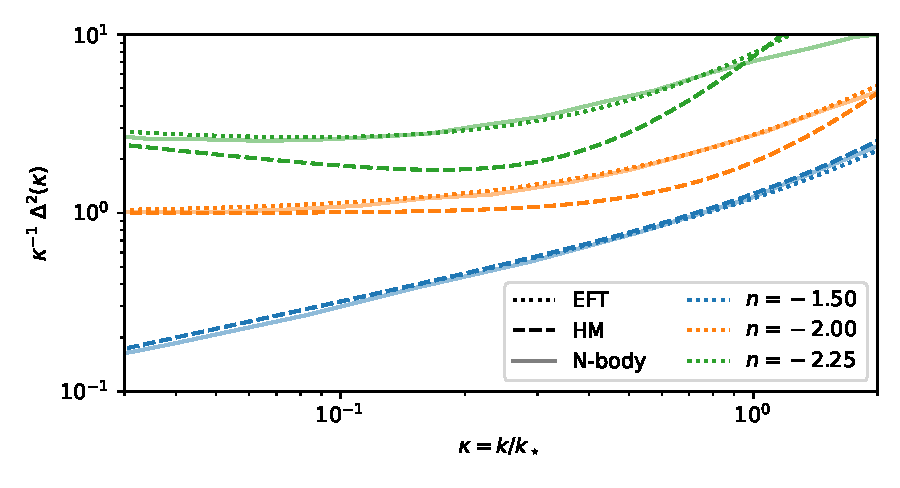
\includegraphics{pt_hm_plot.pdf}}
    \caption{The EFT (dotted) and HM (dasged) dimensionless power spectra, $\Delta^2$, as a function of $\kappa$ for $n=-3/2$, $n=-2$ and $-9/4$ compared to N-body simulations (solid).  For the EFT curves we have adjusted $\alpha$ to match the N-body in the quasi-linear regime ($\kappa=3/4$).  For $n=-3/2$ the HM and EFT agree well with N-body while for lower $n$ the HM predicts a much later onset of non-linearity than EFT (and N-body).  This mismatch gets worse as $n$ becomes more negative.}
    \label{fig:Delta2}
\end{figure}

Figure \ref{fig:Delta2} compares the ``analytic'' halo model to the EFT predictions.  We see that the 1-halo term is not the right description of how structure goes non-linear and this becomes readily apparent for models with more negative $n$, i.e.\ significant large-scale power.  While PT alone does not do very well for $n\approx -3$ the inclusion of the lowest order counterterm is enough to establish agreement with N-body for $\kappa<1$.  This suggests that the mode coupling predicted\footnote{This difference also leads to different predictions for how large-scale flows modify features in the spectrum, such as the baryon acoustic oscillations.  These are also known to be better modeled by PT/EFT than the halo model.} by EFT as the source of the quasi-linear behavior is the more correct behavior.

This result could be important for probes of high-redshift structure, where the non-linear scale moves to a region of the CDM power spectrum with very negative local power-law slope (e.g.\ Fig.~\ref{fig:LCDM}).  It could also be important for using the model to assess higher-order functions or properties of the theory that depend upon correctly modeling the approach to non-linearity.

\begin{figure}
    \centering
    \resizebox{\columnwidth}{!}{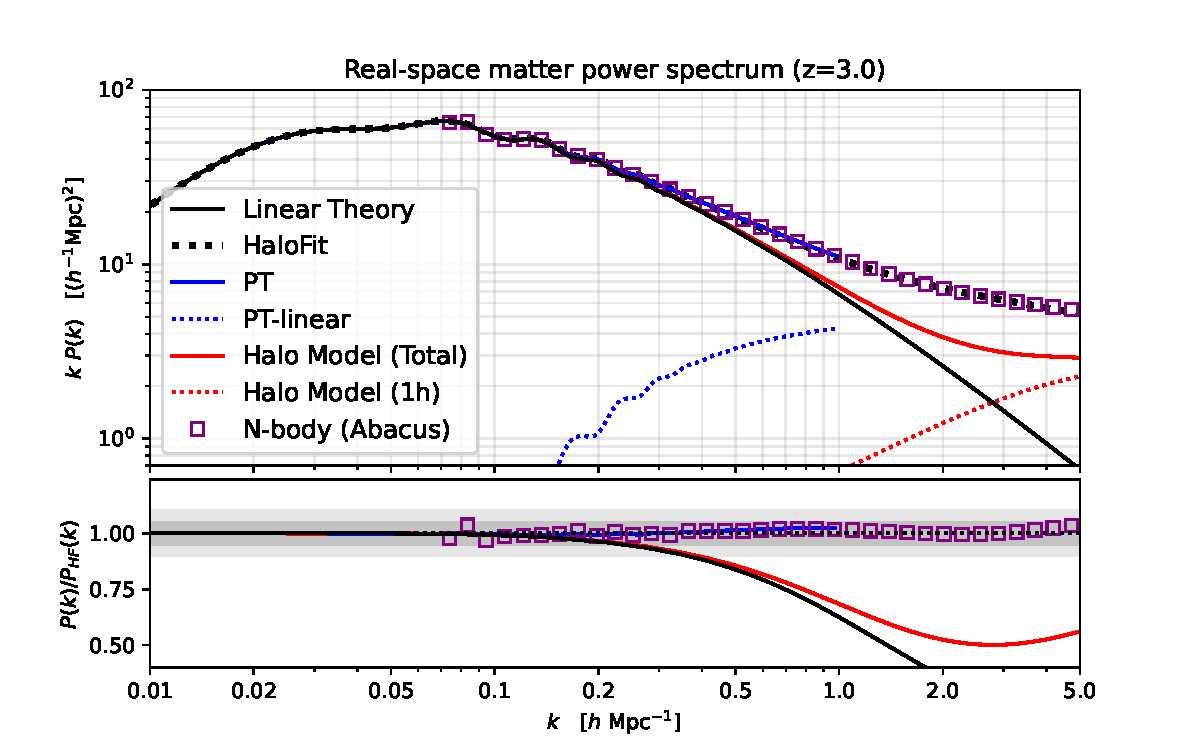
\includegraphics{CCL_halomod.pdf}}
    \caption{An example for $\Lambda$CDM at $z=3$ where the slope of the spectrum near the non-linear scale is more negative (than at $z=0$).  We plot the linear theory power spectrum (solid black), the fitting function of HaloFit/Takahashi (dotted black), the predictions of perturbation theory (blue) with the 1-loop terms separated out (dotted), the halo model prediction from \texttt{pyccl} (red) broken into total and 1-halo contributions (dotted) and N-body results from Abacus (purple squares).  The lower panel shows the ratio to the HaloFit fitting function, with the light and dark grey indicating $\pm 5\%$ and $\pm 10\%$.}
    \label{fig:LCDM}
\end{figure}

\clearpage

\section{Aside: Zeldovich approximation}

The exact expressions for the power spectra of self-similar models in Zeldovich is known (\url{https://arxiv.org/pdf/astro-ph/9604020}).
For example, for $n=-2$
\begin{equation}
    \Delta^2(k) = \frac{16\,a^2 k}{\pi X^2}\left( 1 + \frac{3\pi a^2 k}{4\sqrt{X}}\right)
    \quad , \quad
    X\equiv 1 + 4 a^4 k^2
\end{equation}
If we set $a=1$ and take $k\to 0$ then $\Delta^2_{\rm lin}=(16/\pi)k$ which suggests $k_\star=\pi/16$.  Then
\begin{equation}
    \Delta^2(\kappa) = \kappa + \frac{3\pi^2}{64} \kappa^2
    - \frac{\pi^2}{32}\kappa^3 - \cdots
\end{equation}
and $3\pi^2/64\approx 0.4626$.  The first correction is qualitatively similar to, but not equal to, the perturbation theory prediction.  However the model makes predictions for all scales.


\end{document}
\section{Scratch space}


It is helpful to define a characteristic mass and characteristic radius as the mass for which $\nu=1$ or $\sigma^2(M_\star) = \delta_c^2$ with
\begin{equation}
    \sigma^2\left(R(M)\right) = 
    (k_\star R)^{-3-n}
    \int_0^{\infty}\frac{dx}{x}\ x^{3+n}
    \left[ \frac{3 j_1(x)}{x}\right]^2
\end{equation}
and $R(M) = (3M/4\pi\bar{\rho})^{1/3}$.  The integral can be done in closed form, in terms of $\Gamma$-functions
\begin{align}
    \mathcal{I}_n \equiv
    \int_0^{\infty}\frac{dx}{x}\ x^{3+n}
    \left[ \frac{3 j_1(x)}{x}\right]^2
    &= 9\int_0^{\infty}dx\ x^{n}\, j_1^2(x) \\
    &= \frac{9(1+n)\Gamma(n-1)\sin(n\pi/2)}{2^n(n-3)}
\end{align}
Hence
\begin{align}
    A_\star &= \frac{k_\star^3 M_\star}{2\pi^2 \bar{\rho}}
    = \frac{2}{3\pi}\left(k_\star R_\star\right)^3 \\
    \gamma &= 2^{3/(3+n)} \pi^{-1/2}\ \Gamma\left[ \frac{1}{2}+\frac{3}{3+n} \right]
\end{align}
where $\gamma$ is 1 for $n=0$ but 15 for $n=-2$.\newline
\underline{Note} this also allows us to define $R_\star$ in terms of $k_\star$ but we want to be a bit careful about whether $\sigma(R_\star)=1$ or $\sigma(R_\star)=\delta_c$.  Could differ depending upon usage.

Defining $\nu=[\delta_c/\sigma(M)]^2$ we can write the mass and multiplicity functions as
\begin{equation}
    f(\nu)d\nu \equiv \frac{M}{\bar{\rho}}  n_h(M) dM
    = \frac{e^{-\nu/2}}{\sqrt{2\pi\nu}}
\end{equation}
leading to $b_h(\nu) = 1 + (\nu-1)/\delta_c$.


\begin{equation}
    \Delta^2_{1h} = k^3/(2\pi^2 \bar{\rho}^2) \int dM n_h M^2 y^2
    \quad , \quad
    \Delta^2_{2h} = \Delta^2_{\rm lin} + \mathrm{corrections-from-}y.
\end{equation}
Can rewrite 1h as
\begin{equation}
  \frac{k^3}{2\pi^2 \bar{\rho}^2} \int d\nu f(\nu) \frac{\bar{\rho}}{M}  M^2 y^2
 = \frac{k^3M*}{2\pi^2\bar{\rho}} \int d\nu f(\nu) m(\nu)
\end{equation}
as written in the paper.  Since $\nu=m^{(n+3)/3}$ this times the PS multiplicity function presumably gives the gamma expression above [Check].

Note that the N-body results use $k\,R_{NL}$ as their $x$-axis.  We we need to know $k_\star\, R_{NL}$.  They define $\sigma^2(R_{NL})=1$, thus
\begin{equation}
    k_\star\,R_{NL} =  \mathcal{I}_n^{1/(n+3)}
\end{equation}

\end{document}
